%!TEX root = series of tubes.tex
\section{\systemname - A Tool for Pipe Design}
To allow makers to design novel objects with pipe-powered interfaces, we created a tool, \systemnamenospace, to add pipe geometries to arbitrary 3D models. Pipe design is non-trivial.  Independent pipes should not intersect inside an object lest their contents be unintentionally mixed.  To permit easy insertion of media after printing, pipes should have smooth bends.  Pipes, in general, need to avoid objects' surfaces to prevent fluid leakage when printed by hobbyist-grade machines.  Finally, for designing path-constrained pipes that follow a user-specified path, we must ensure certain characteristics of that path (e.g., that it is connected). 
%\george{pipes are hard.  not sure we convinced readers by now that they are worth the effort.  maybe this has to happen more in the intro.  the example objects section is still a few pages away.}

\systemname allows users to design pipes in two ways. In one, they can select exterior anchor points on their objects; the tool then creates complete point-to-point routings using A* path search and physical rod simulation (see Figure \ref{fig:tool-process-exterior}). In the other, users can import vector art describing desired interior paths (see Figure \ref{fig:tool-process-interior}).  \systemname then creates a single path that follows the input shape using edge graph manipulation and Euler tour generation.  We thicken these routes to create pipes.  The resultant pipes are subtracted from the original mesh using voxelization and remeshing. Our tool is implemented in C++ as an extension to Meshmixer, a consumer 3D mesh editing tool~\cite{Schmidt-meshmixer}.

\subsection{Exterior Terminals}

% Designing objects which, for example, are touch sensitive in particular areas or contain electronic components, requires precise location and sizing of pipe endpoints.  The interior of these pipes should have as large a bending radius as possible so that post-print insertion of solid or viscous media is easier.
To create endpoint-constrained pipes, in which the location and shape of exterior connection points matters, a brush tool is used to specify a pair of points on the mesh's surface. The system automatically routes the pipe, and displays a preview.  Using sliders, the user can independently adjust the starting and ending radii of the pipe.  This is useful for, e.g, our breathing bunny (Figure \ref{fig:examples}b), whose pipes must fit a piece of hardware on one end, but on the other end should have as large an interactive surface as possible.

\begin{figure}[h!]
\centering
    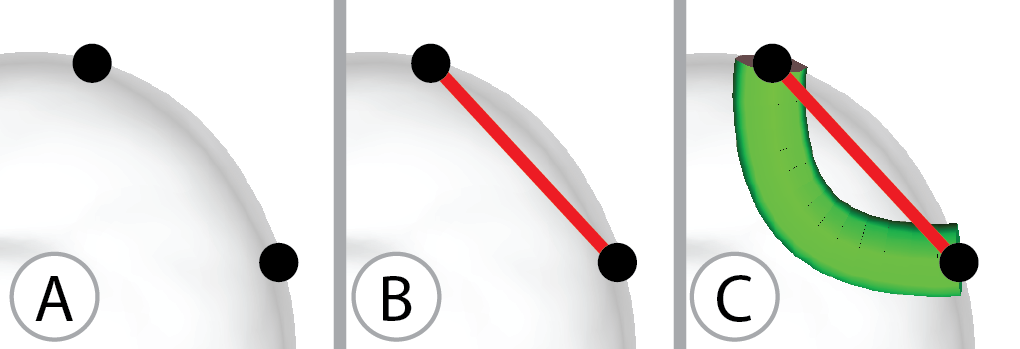
\includegraphics[width=3.4in]{figures/exterior.png}
\caption{In a), an example mesh with exterior connection points selected.  The smoothed A* routing (b) is drawn in {\color{red}red}.  In {\color{tovi}green} is our physically-based rod after simulation (c).}
\label{fig:tool-process-exterior}
\end{figure}

\subsubsection{Routing Algorithm and Physical Simulation}
Given two points, we first find a path between them using the A* search algorithm on a voxel representation of the object~\cite{Hart-Astar}. A* finds a least-cost path through a graph of nodes given a cost function. Our graph comprises the grid of voxels as nodes, with edges between adjacent nodes; our path cost is based on the Euclidean distance to the selected end point. In this formulation, the routed path is naturally constrained to stay within the object boundaries.
%; for each point it tags the distance from the start (e.g., startPoint = 0, startNeighbors=1, ...).  Once the end point is reached, we backtrack through tagged points, always moving to a lower-valued point. \bjoern{find a clearer way to express this?}

Our A* pathfinding produces the \emph{shortest} path, but in many cases
we require a smoother path to aid insertion of the desired medium, such as a threadable wire.
In addition, the distance from the surface is not taken into account in the A* search and pipes may thus be routed along surface contours, which may cause leakage or structural deficiencies.

We solve this problem via physical simulation. We create a straight virtual 
wire (a 3D polyline or \emph{discrete rod}), and then set its initial position 
as our A* path.
Running the physical simulation allows the wire to attempt to return to
a straight configuration, while satisfying the user-selected endpoint position constraints.  In addition to user constraints, we require that the rod be perpendicular to the surface at its ends to prevent the terminals' shape from deforming.

The wire is modelled as a \emph{discrete rod}: a 3D poly-line with a bending 
constraint between adjacent segments. Our simulation is based on an
implementation of Position-Based Dynamics (PBD)~\cite{Muller07}, with all constraints
modelled as penalty forces. To keep the rod inside the
mesh, we compute a discretized distance field, then constrain the
rod to stay within our offset shell using a simple penalty force.

%In the case of multiple initial paths, we solve for each smoothed path sequentially.\bjoern{Why would we ever end up with multiple paths here? It thought we processed each path by running it through the (A*-PBD-Cutout) pipeline. So this step should only ever see one path, no?}\tovi{agree this is misleading, I think it can be removed since we talk about multiple pipes in a later paragraph}

PBD simulations rarely converge to a steady state, so we simply halt after a fixed number of timesteps (250). Our voxel grid currently uses a resolution of 128x128x128 voxels, which enables interactive operations, but this parameter can be adjusted for different model requirements. The simulation takes about a second for most of our examples.

\subsubsection{Multiple Pipes}
Pipes are routed and cut out of the mesh serially. This prevents pipe intersections: once a pipe has been cut out of the mesh, it cannot be part of valid routes in any future pipe routing operation. After solving for a path, we add it as a constraint to the system, generating
a penalty force that pushes additional paths away from it.  However, we do not currently track all pipes for global optimization: we greedily select the best routing per pipe. 

\subsubsection{Pipes with Multiple Endpoints}
To allow designers to create pipes with multiple endpoints (e.g., the star topologies in Figure \ref{fig:examples}a), we use one surface position per pipe and a central fixed endpoint that the user can interactively position (see Figure~\ref{fig:boat-star}).  The user can connect several pipes, hitting a key to add each in sequence and positioning them with the mouse.  The pipes route as normal.

\begin{figure}[b]
\centering
    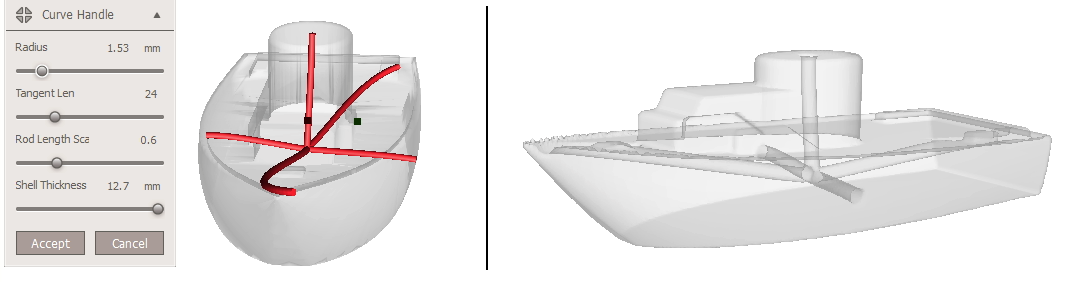
\includegraphics[width=1.0\columnwidth]{figures/boat-star.png}
\caption{Left: Users can interactively position connection points for pipe topologies; they can also adjust pipe diameter and rod parameters. Right: Resulting model with cut pipes.}
\label{fig:boat-star}
\end{figure}

\subsection{Interior Paths}

For path-constrained pipes, the route of the pipe must conform to a desired shape. A maker can import a vector graphics file (such as SVG) describing the path she wants for her pipes: all lines in this input file are interpreted as desired pipe components for the final artifact.  Using sliders, she can change the pipes' radius.  A preview is provided to show the radius and location of the cut, and the maker can align her model as appropriate.

In some cases, such as for the neon sign in Figure \ref{fig:tool-process-interior}, a single path must pass through a set of disconnected path segments (i.e., all letters in the word ``UIST'' ).  \systemname leverages graph theory algorithms to generate this single path, as described below.  Without endpoint constraints, the path's exit(s) from the model are defined by the SVG: the maker can see where the path exits the model and translate the cut according to her desired outcome.

\begin{figure}[h!]
\centering
    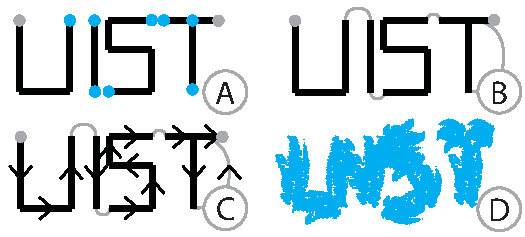
\includegraphics[width=3.4in]{figures/interior.pdf}
\caption{An input vector graphics file with the start and end points highlighted in {\color{gray}gray} (a) and the points which cannot be tubed as drawn highlighted in {\color{blue}blue} (b).  The connected graph created by our software (c) and the resulting Euler tour (d) permit insertion of media post-print.}
\label{fig:tool-process-interior}
\end{figure}

\begin{figure}[h!]
\centering
    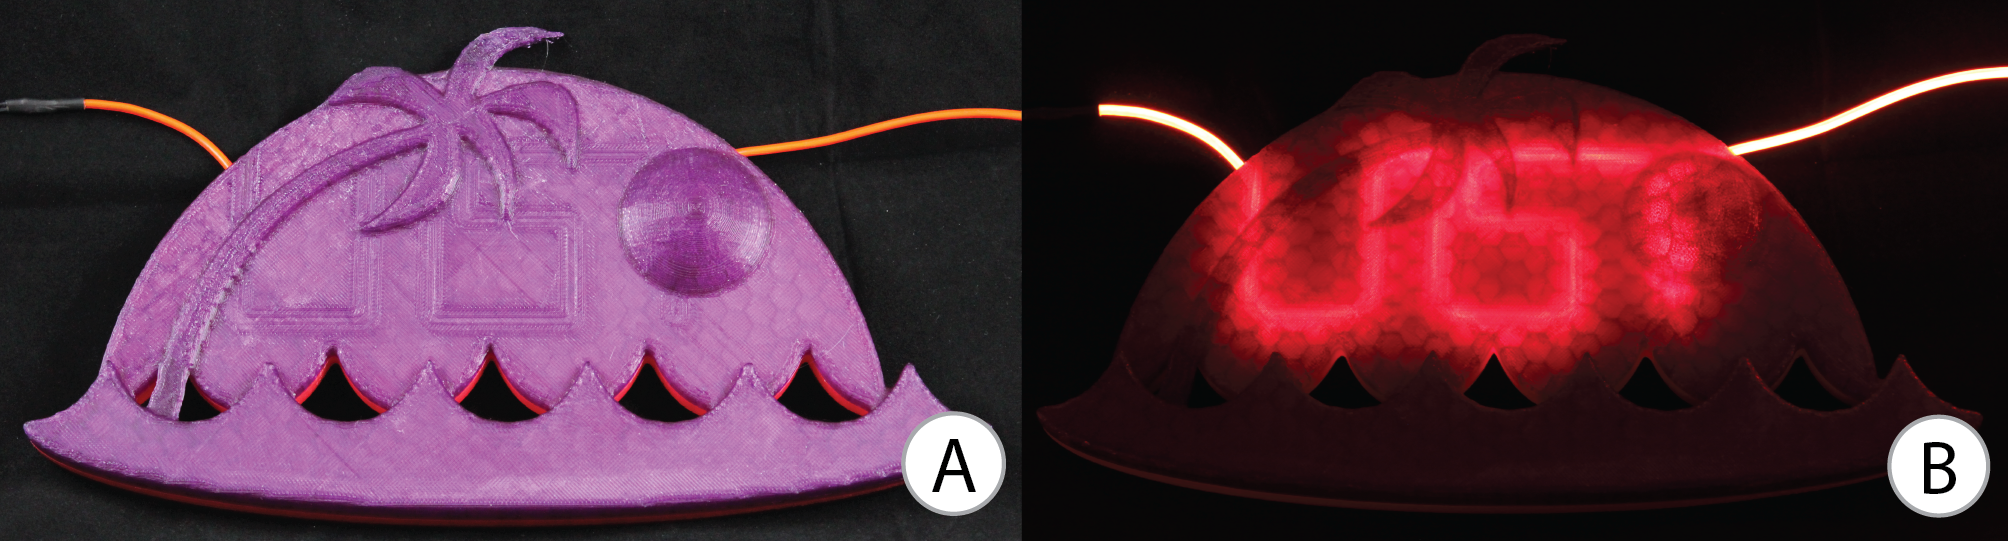
\includegraphics[width=3.4in]{figures/uistphotos.png}
\caption{Our neon sign built using the process above.  (a) shows the unlit sign, and (b) shows it lit.}
\label{fig:UIST}
\end{figure}

\subsubsection{Routing}
%To allow for a single path through a pipe for post-print media insertion, we need to find a semi-Eulerian graph of which a user's input graphics are a subset, and subsequently find an Euler tour on that graph. \bjoern{just said the same thing in the last section.}
%

%In graph theory, a semi-Eulerian graph is one which has exactly two edges of odd degree.  This kind of graph supports an Euler tour: a path that travels every edge exactly once, beginning and ending at the two nodes of odd degree (in this case, the user-selected start and end nodes).  We create a graph based on the user-specified geometry data, with edges for all line segments; then add edges to connect graph components and make graph the semi-Eulerian.  We find an Euler tour on the modified graph, and thicken the path to create pipes.  
Our technique for routing this path is inspired by work in generating continuous line illustrations from images~\cite{Wong-continuousline,Bosch-tsp}.  Our routing problem is a version of the Chinese Postman Problem\footnote{The CPP is also known as the route inspection problem: \url{http://en.wikipedia.org/wiki/Route_inspection_problem}}, in which we wish to traverse all edges of the graph described by the user's input, much as a postman needs to walk along every road at least once to deliver mail.  In our relaxation, we allow the creation of new edges (i.e., the postman may jump from building to building in addition to using existing roads).
%
%If path components are disconnected, we create edges that connect them; additionally we can create edges connecting odd-degree vertices rather than simply retracing existing edges.  In the final artifact, all created edges will be blocked out by dark material so the inserted medium is not visible (see Figure \ref{fig:tool-process-interior}).  
%We offer a short algorithm here, with a more mathematically precise definition and associated proof in supplemental materials appendix.

{\bf Setup:} We first add a temporary edge that connects the user's desired start and end points, and create a full Eulerian graph.  This edge is removed at the end to yield a semi-Eulerian graph that can be threaded after printing.

{\bf Connect disconnected components:} To connect disconnected subgraphs, we find minimum Euclidean distance vertex pairs spanning two subgraphs, and greedily add edges to such pairs until all subgraphs are joined into a single graph.
%To connect disconnected subgraphs in the input, each disconnected subgraph's vertices and edges are contracted to a single vertex.  Each subgraph-vertex has no outgoing edges, as the expanded subgraphs are disconnected.  We then add one edge from each subgraph-vertex to each other subgraph-vertex, whose weight is the minimum Euclidean distance between any two vertices in the expanded subgraphs.  We greedily select the smallest weight edges until all subgraphs are joined into a single graph.  We re-expand the subgraphs.

{\bf Eulerization:} In order to make our graph Eulerian, we consider all odd degree vertices in the connected graph and make a clique of potential edges based on distance.  We greedily add edges between the odd nodes until no odd nodes remain.  Finally, we remove our temporary edge, changing the graph from Eulerian to semi-Eulerian.  This is a connected, semi-Eulerian graph which contains all edges in the input.
A lower total weight matching may be possible by connecting components and ensuring node evenness together in a global process, as well as by using minimum-weight matching rather than greedy selection, however this optimization is not crucial for our purposes.

{\bf Euler Tour:} To find an Euler tour, we use Fleury's algorithm\footnote{\url{http://en.wikipedia.org/wiki/Eulerian_path\#Fleury.27s_algorithm}}, with a modification to preserve continuity: at a given node, from multiple candidate edges, we prefer the edge(s) with the smallest angular deviation from the incoming edge (i.e., we prefer to pass straight through a node, if possible).  This minimizes turns in the final artifact, which eases support material removal and assembly.  Our EL wire in Figure \ref{fig:UIST} follows an Euler tour through the input nodes.

\subsubsection{Edges that Intersect in the Plane}
We do not currently redirect edges that intersect in the plane.  Because we have a 3-dimensional canvas in which to work, it would be possible to push overlapping paths into the third dimension.  However, we leave this to future work.  For our specific applications so far, it has been unnecessary.

\subsection{Mesh Modification}
After the maker hits ``Accept'' on her preview, we must cut pipes out of the input mesh.  At this stage, we verify whether the new pipe will intersect the surface or an existing pipe, and if so display a warning message suggesting that she should consider a smaller radius.
Our basic strategy for the cut is to create a polygonal tube by sweeping a profile polyline
along the path, and subtract the tube from the mesh. We only use circular profiles
in our examples, but clearly any other profile could be used. 
We allow different start and end radii, selected by the maker in the previous step, which are linearly interpolated along the path.

To avoid the complexities of direct mesh booleans, we construct a discretized volumetric (i.e., voxel-based) representation of the original mesh and the tube mesh.  Boolean subtraction is trivial in such representations.  We specifically use narrow-band level sets~\cite{Museth04}, which represent the surface as the zero iso-contour of an
approximate distance field.
We then use marching cubes~\cite{Lorensen87} to produce the final mesh for printing.
This strategy does incur some resampling artifacts, however so does the 3D printing, and compared to the print process, the time required to voxelize at high resolution is inconsequential.
Since we have a distance field, we can easily introduce useful effects, such as the
ability to add a thin membrane ``cap'' over the end of a tube. 
This is accomplished by applying a standard ``thicken'' operation to the level set version
of the initial mesh, intersecting with a sphere placed at the tube endpoint, and then performing
a boolean union with the initial shape-minus-tube result (see Figure \ref{fig:cap}).
A straightforward extension would be to add or subtract additional elements at
the tube endpoints.

\begin{figure}[t]
\centering
    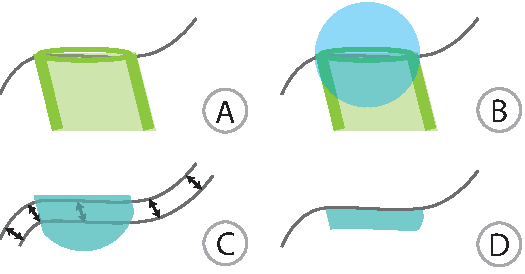
\includegraphics[width=3.4in]{figures/cap.pdf}
\caption{The process to ``cap'' the end of a pipe.  In (a), a pipe end is placed on the surface of the mesh.  In (b), we create a sphere whose radius is slightly larger than the radius of the pipe, centred at the tube's endpoint.  In (c), we consider the intersection of the sphere and the pipe, and create an offset surface of the mesh.  Finally, in (d) we intersect with the offset surface.  This is kept as a cap for the pipe in mesh subtraction.}
\label{fig:cap}
\end{figure}

\section{Fabrication Techniques}
Several pragmatic concerns arise when fabricating models with hollow pipes and cavities on additive manufactuing machines. Pipes will frequently lead to overhangs (where an underlying supporting layer has a smaller footprint than the subsequent layer).
%Beyond design, the tubes must actually be printable to be useful.  
%When geometries contain overhangs, as there may be in designed pipes and cavities, 
To allow overhangs, 3D printers lay down support material that must be later removed from the model.  This removal process can be time-intensive and challenging.  The physical fabrication process used by different machines gives rise to differing strategies for avoiding support material or easing its removal.  We next discuss techniques for fused deposition modeling (FDM) machines, such as the Makerbot\footnote{\url{http://makerbot.com}} and multi-jetting machines such as Objet\footnote{\url{http://stratasys.com}}, as well as powder-based machines (e.g., ZCorp\footnote{\url{http://3dsystems.com}}) and those that use stereolithography (e.g., Form 1\footnote{\url{http://formlabs.com}}).

\subsection{Fused Deposition Modeling}
FDM machines lay down lines of extruded plastic filament on top of each other: this allows {\em stepover}, when a layer of plastic is laid slightly offset from the layer below it, and {\em bridging}, when plastic is laid across a gap between two surfaces.  For a layer to fix correctly to its supporting layer, roughly half of the filament needs to overlap.  This means that overhangs without added support material can be approximately $45^{\circ}$, and although cylinders (e.g., pipes) and spheres violate this in some places they can be printed support-free. The colored models in Figure \ref{fig:teaser} were produced on a Makerbot FDM without any support structures inside the pipes.

On single-material hobbyist FDM printers, support structures are built using the same material as the model. Such support may be impossible to remove from internal cavities.  Meshmixer has a built-in tool for minimizing support for FDM prints; it re-orients the part to keep as much surface area as possible within the 45 degree constraint.  In future work we would like to explore a tool in which a user can select surfaces (pipes) that should be prioritized for support avoidance.

\subsection{Multi-Jetting}
On multi-jetting machines, bridging is not possible and stepover potential is much less, because the machine is laying down droplets of liquid that are later UV cured.  Unsupported overhangs can be approximately $14^{\circ}$ on our Objet printer.  Multi-jetting and higher-end FDM machines use a secondary support material that must be manually removed afterwards. Some support can be melted out (Projet wax material); other support can be dissolved in lye or blasted with high-pressure water. Complex pipe geometries can make water blasting impossible and other processes more labor- and time-intensive.  All models in Figure \ref{fig:teaser}b required support material removal post-print: the neon sign and maze were additionally cut into two pieces to give better access to the support.

\subsection{Powder-based and Stereolithography}
Powder-based and stereolithography (SLA) machines work with a bed of powder or liquid, respectively.  The material at the surface is fused together via glue droplets (for powder) or a UV laser (for SLA).  The remaining powder or liquid serves as support for the model.  These types of printers are perhaps even more suitable for pipe creation than either FDM or multi-jetting printers, as the supporting liquid or loose powder is simpler to remove than structural plastic or UV cured resin.  We hope to experiment with them in the future.

\subsection{Model Assembly}
For especially complex geometries, models can be ``cut up'' into multiple pieces that can be assembled to avoid support deposition or at least ease material removal. This is undesirable as it means more time spent in assembly post-print, and additionally a cut pipe may not be fluid-tight any longer.  An automatic tool for this task might be beneficial, however it is outside the scope of this work.